\section{MNIST left-right cross-reconstruction}
\label{sec:mnist}
\begin{figure}[!h]
\centering
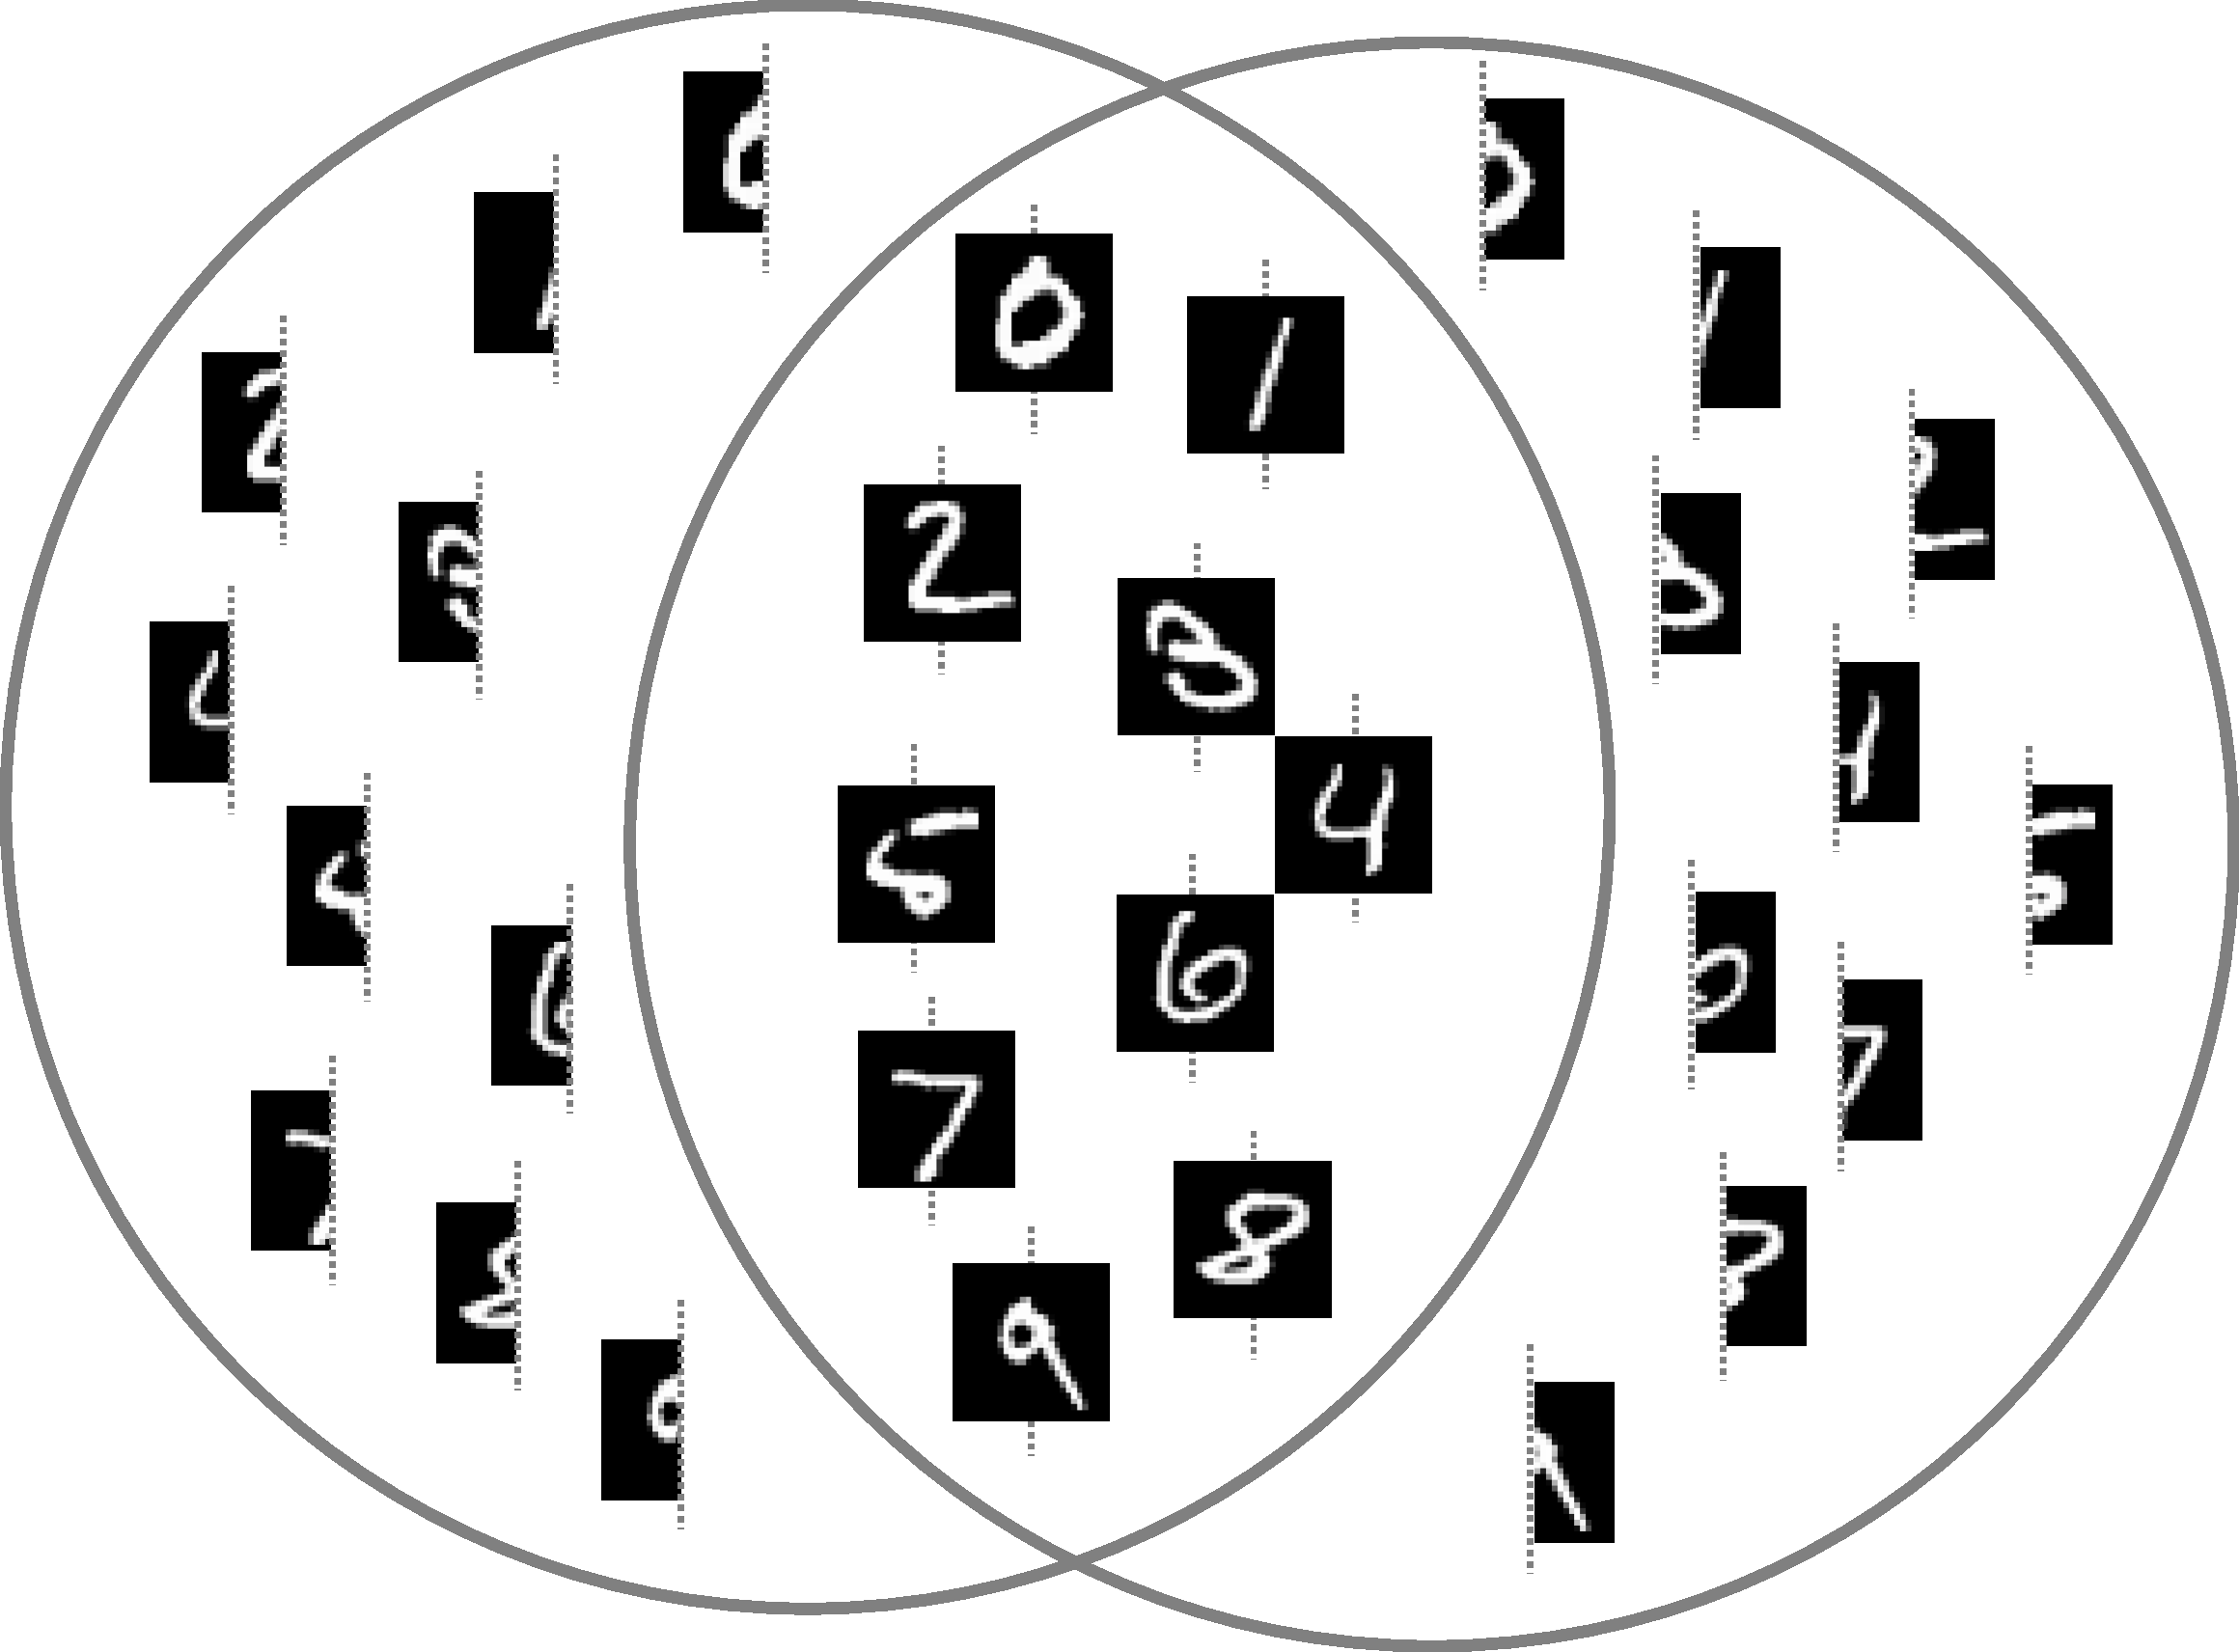
\includegraphics[width=0.8\columnwidth]{./tex/fig/mnist_scheme.pdf}
\caption{
	Pictorial example of training imaging dataset with two views, named \textit{left} and \textit{right} views.
	In this case we have 30 independent observations:
	$10$ with left-views only; $10$ with right-views only; $10$ with complete views.
	The fraction f of observations with complete views is:
	$f = 1/3$.
}
\label{fig:mnist_scheme}
\end{figure}
%
\begin{figure}[!h]
\centering
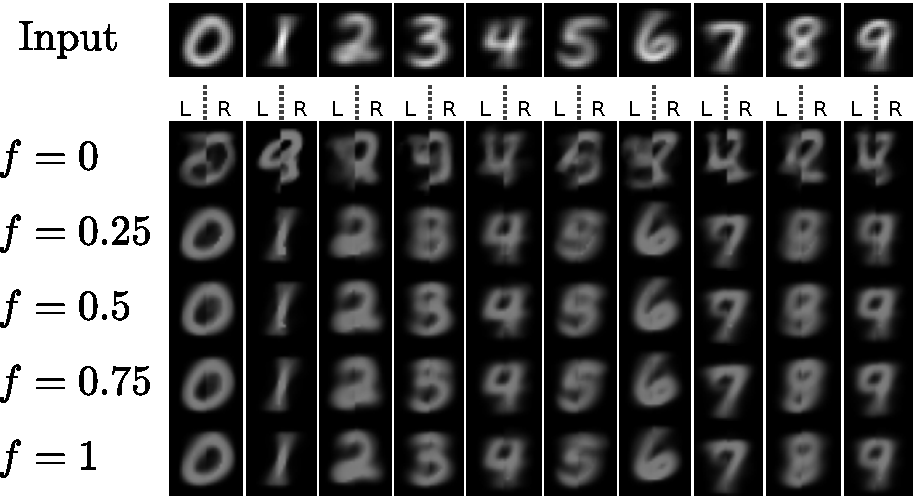
\includegraphics[width=0.8\columnwidth]{./tex/fig/mnist_half.pdf}
\caption{
	Reconstruction of test-set digits when models are trained with an increasing fraction ($f$) of observations with complete-views.
	The left side of each digit is inferred from the input right side and \textit{vice versa}.
}
\label{fig:mnist_half}
\end{figure}


In this section we describe our results on jointly modeling the left and right halves of hand-written digits coming from the MNIST dataset \citep{mnist}, which consists of $60k$ train images and $10k$ test images.
To simulate a two-views dataset, the original $28 \times 28$ grayscale images were divided into a left and a right half, each one consisting in a $28 \times 14$ grayscale image ($392$ features).
To simulate a dataset with missing views, we adopted the same procedure described in the previous section, by controlling the fraction $f$ of observation with complete views.
In \figref{fig:mnist_scheme} we show a small ($n=30$) training dataset created with $f=1/3$.
For our true experiment we took all the $50k$ training images and we randomly removed the left and right view until reaching values of $f \in \{0, 0.25, 0.5, 0.75, 1\}$.
We adopted a deep architecture with $4$ layers encoders, having ReLU activation functions and dimensions $392-800-800-16$ in the encoding and $16-800-800-392$ in the decoding path,
similar to those used by \cite{dcca1} and \cite{dcca2} for a similar task.
We adopted a Bernoulli likelihood for the decoders and we trained our model with a mini-batch size of $1000$ for $1000$ epochs, after setting up the Adam optimizer with a learning rate of 0.001.
Training was repeated $5$ times, by changing the initialization random seed.

\subsection{Results}
In \tabref{tab:mnist_half} we show the Mean Squared Error (MSE) and Negative Log-Likelihood (NLL) when predicting the left halves from the right ones and \textit{vice versa} in the testing set.
In \figref{fig:mnist_half} is possible to visually inspect these predictions.
Results are consistent with the ones in \figref{fig:synthetic_benchmark_pred_box}, where a value of $f = 0.25$ is enough to reduce the prediction error on testing data-points at the level of the ideal case ($f=1$).
\begin{table}[h]
\centering
\caption{
	Mean squared error (MSE) and negative log-likelihood (NLL) measured on the reconstructed MNIST test set (mean (st.dev.), the lower the better).
	The left halves of the images were used to infer the right ones, and \textit{vice versa}.
	Results stratified by $f$, the fraction of observations with complete left and right views in the training set.
}
\label{tab:mnist_half}
\resizebox{\columnwidth}{!}{
	\begin{tabular}{llllll}
	\toprule
	f                &             0.00 &           0.25 &           0.50 &           0.75 &           1.00 \\
	\midrule
	MSE             &     35.21 (1.64) &   19.43 (0.44) &   19.36 (0.18) &   18.82 (0.24) &   19.21 (0.84) \\
	NLL              &   221.96 (20.41) &   80.25 (1.39) &   80.12 (0.81) &   78.19 (0.77) &   79.54 (2.86) \\
	\bottomrule
	\end{tabular}
}
\end{table}


